\documentclass{article}
\usepackage{graphicx}

\usepackage{color}
\definecolor{color02}{rgb}{0.00,0.00,1.00}

\begin{document}

\section{Summary}

SpaghettiLens is a tool developed by Rafael Kueng {\small{}[1]} that makes it possible 
for SpaceWarps volunteers to easily model Gravitational Lenses (GL). It is a simple 
web user interface that requires very little training to use. With the release 
of SpaghettiLens v1.4.1 it became possible for volunteers to work together, refining 
each other models, in order to come up with the most successful model for a single 
GL candidate. 

\section{Why is it Necessary to Model Lens Candidates?}

When a SpaceWarps volunteer flags an object as being a possible GL candidate, it 
is necessary to do follow up work to determine if it is, in fact, a worthy candidate. 
If we can successfully create a simple model that has the physical characteristics 
of the object concerned, it suggests that the object could indeed be a lens.

\section{How did we go about collaborative modelling?}

The SpaceWarps Science Team {\small{}[2]} selected candidate {\color{color02} \emph{ASW0004dv8}} 
 [Fig.1] as being the initial subject for collaborative modelling. A basic model 
({\color{color02} \emph{4516}}) [Fig.2] was generated and it was expected the volunteers 
would continue to refine this model.

\begin{figure}
\centering
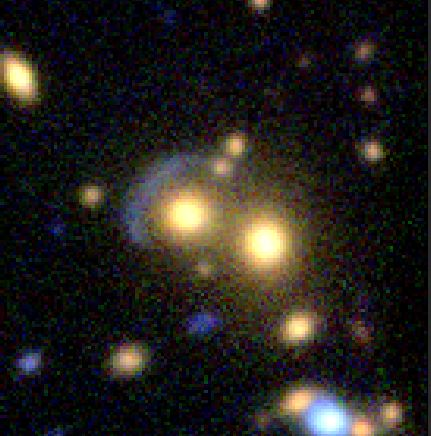
\includegraphics[width=136pt]{fig/simsModeling-fig001.jpg}
\caption{Figure caption.}
\end{figure}

\begin{figure}
\centering

\includegraphics[width=184pt]{fig/simsModeling-fig002.png}
\caption{Figure caption.}
\end{figure}

As nothing like this had been done before, we had expected there to be initial 
problems. User apathy / lack of collaboration were a concern. Once a manual system, 
using SpaceWarps Talk, had been put into place to report the changes a volunteer 
had made, the outcome of those changes, and improvements the volunteer would like 
to see to the model - things went smoother. With the addition of Google+ spread 
sheet {\small{}[3]} to track our changes, managing the project became easier.

In total, 47 models were posted - this does not include the countless models that 
were rejected by the volunteers concerned. The vast majority of the models posted 
were descendants {\small{}[4]} of the initial model, the geneology [Fig.3] of the 
initial model makes interesting viewing. It is important to note, only models posted 
by their owners in the thread {\small{}[5]} on SpaceWarps were included.

\begin{figure}
\centering
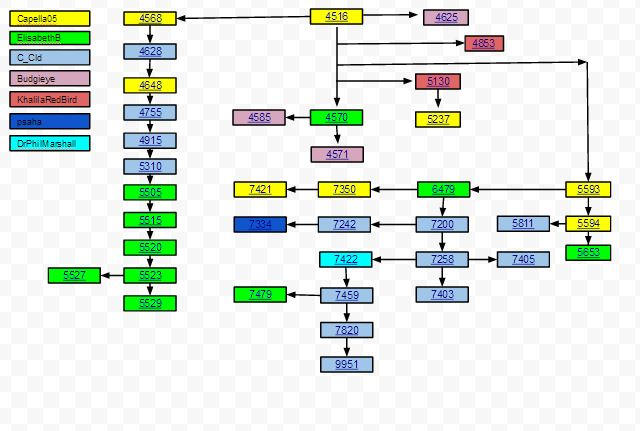
\includegraphics[width=500pt,angle=90,origin=c]{fig/simsModeling-fig003.jpg}
\caption{This should be the caption for \texttt{fig/simsModeling-fig003.jpg}.}
\end{figure}

\section{What determines a successful model from a failure?}

When analysing the output of a model there are several things we look for; are 
the lines of the contour plot smooth and uncomplicated [Fig.4]? Is the Mass Distribution 
clean or does it resemble a chessboard [Fig.5]? Finally, does the Synthetic image 
resemble the lensed object [Fig.6]? If we can say yes for all of the above, we 
can deem the model a success. For the purposes of this letter we will ignore other 
output from SpaghettiLens. Each of the images represented below are from different 
models that were generated within this project, and are used to represent the criteria 
we were looking for. 

\begin{figure}
\centering
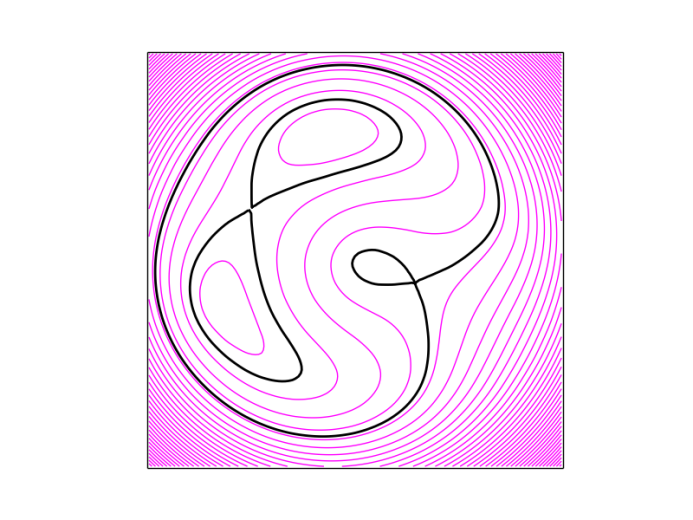
\includegraphics[width=300pt]{fig/simsModeling-fig004.png}
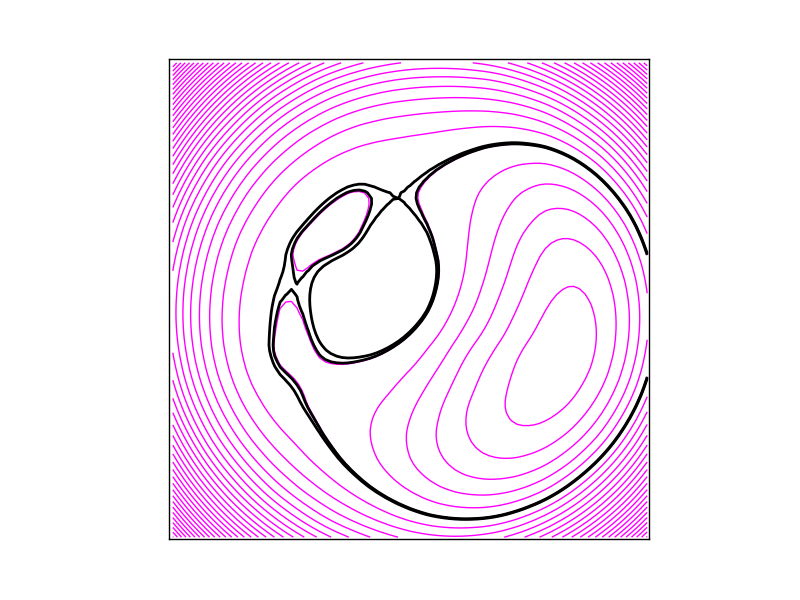
\includegraphics[width=300pt]{fig/simsModeling-fig005.png}
\caption{Contour Plot: {\color{color02} \emph{Success}}
  {\color{color02} \emph{Failure}}}
\end{figure}

\begin{figure}
\centering
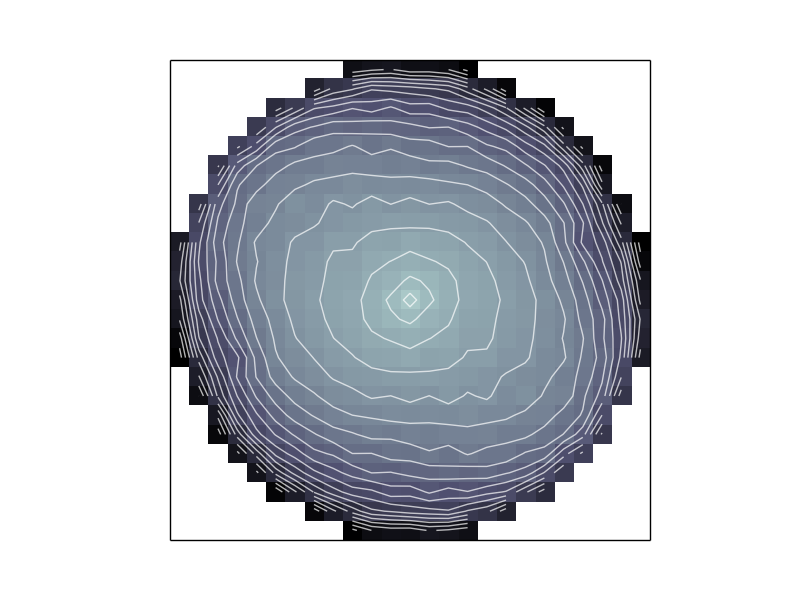
\includegraphics[width=300pt]{fig/simsModeling-fig006.png}
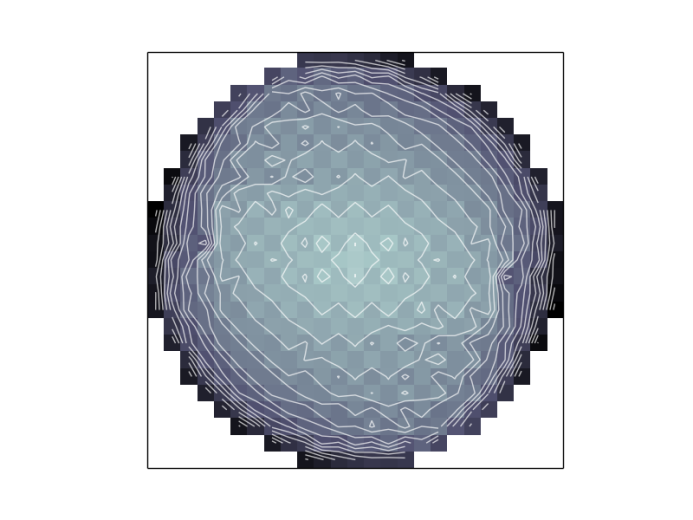
\includegraphics[width=300pt]{fig/simsModeling-fig007.png}
\caption{Mass Distribution: {\color{color02} \emph{Success}}
  Mass Distribution: {\color{color02} \emph{Failure}}}
\end{figure}

\begin{figure}
\centering
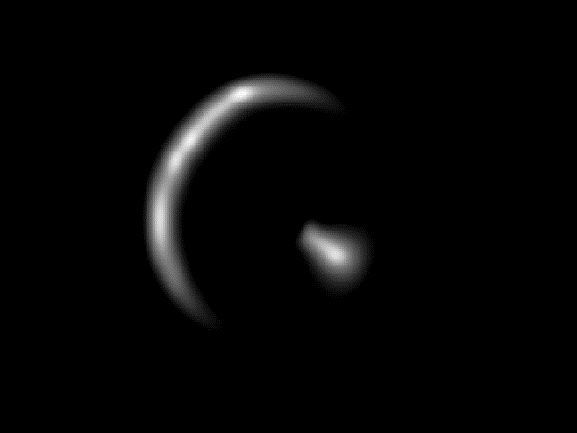
\includegraphics[width=300pt]{fig/simsModeling-fig008.png}
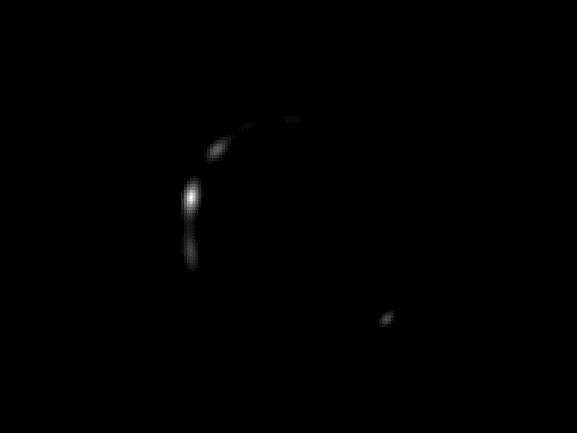
\includegraphics[width=300pt]{fig/simsModeling-fig009.png}
\caption{Synthetic Image: {\color{color02} \emph{Success}}
  Synthetic Image: {\color{color02} \emph{Failure}}}
\end{figure}


\section{Where we able to reach consensus on a single successful model?}

In a word, No.

Do we consider this a failure? Not necessarily. 

By the end of the project we have narrowed down the list to 12 convincing models. 
We have refined techniques that can be used to move collaborative modelling forward, 
and in the process, the skills of the existing modellers have been improved. I 
was recently asked what I hoped to achieve by writing this letter - the answer 
is easy; if we can attract more Zooniverse volunteers to lens modelling, and dispel 
the myth that it is the preserve of Astrophysicists', it is a job well done. 

{\small{}Clicking on an image below will navigate you to the corresponding model 
result page.}

\begin{figure}
\centering
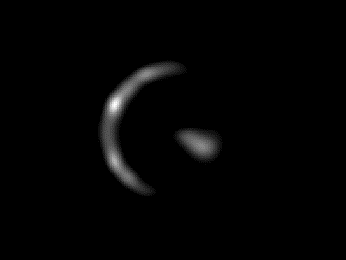
\includegraphics[width=113pt]{fig/simsModeling-fig010.png}
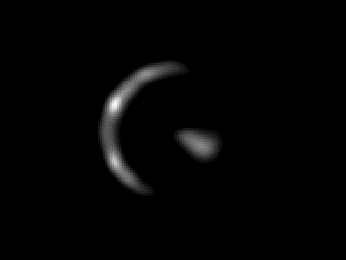
\includegraphics[width=113pt]{fig/simsModeling-fig011.png}
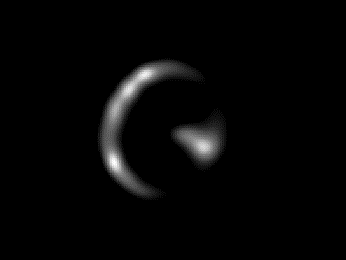
\includegraphics[width=113pt]{fig/simsModeling-fig012.png} \\
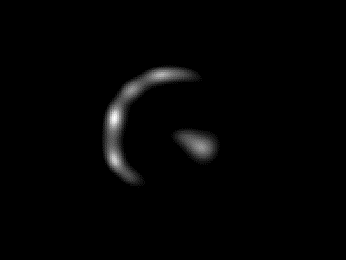
\includegraphics[width=113pt]{fig/simsModeling-fig013.png}
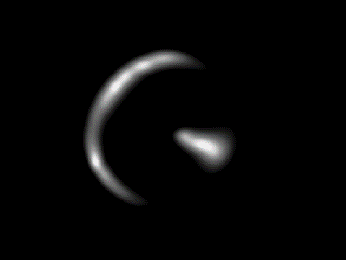
\includegraphics[width=113pt]{fig/simsModeling-fig014.png}
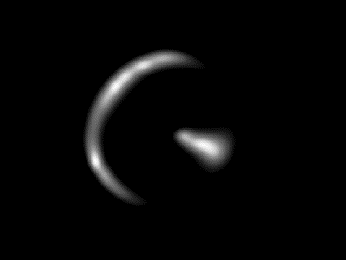
\includegraphics[width=113pt]{fig/simsModeling-fig015.png} \\
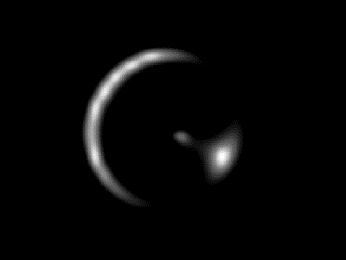
\includegraphics[width=113pt]{fig/simsModeling-fig016.png}
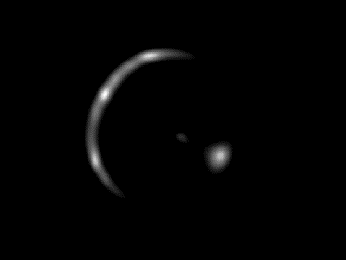
\includegraphics[width=113pt]{fig/simsModeling-fig017.png}
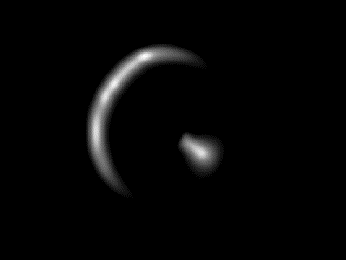
\includegraphics[width=113pt]{fig/simsModeling-fig018.png} \\
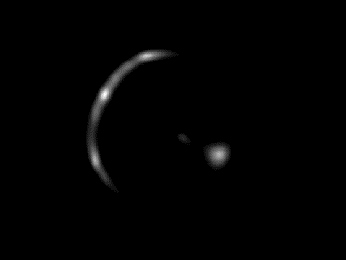
\includegraphics[width=113pt]{fig/simsModeling-fig019.png}
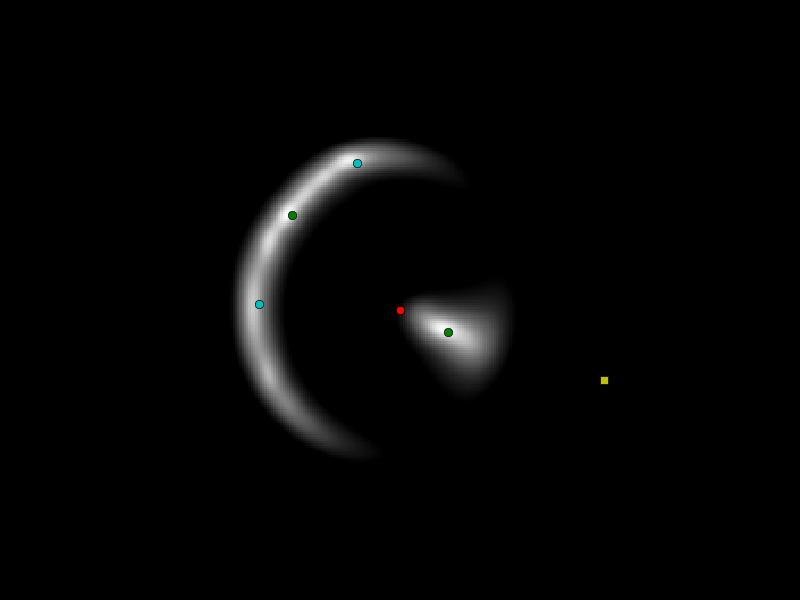
\includegraphics[width=113pt]{fig/simsModeling-fig020.png}
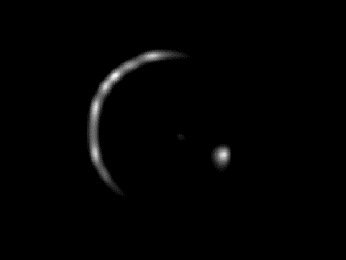
\includegraphics[width=113pt]{fig/simsModeling-fig021.png}
\caption{Figure caption.}
\end{figure}

\section{Feedback and moving collaborative modelling forward.}

With all previous Zooniverse projects {\small{}[6]} volunteers would independently 
classify images and at the end of the project, mass consensus would determine the 
result. The Science Team would interpret the results and present a paper.  

When we started this project it was not clear whether the volunteers would prefer 
to work in a team or independent of each other - It appears we have a happy medium. 
On the positive front, we enjoy learning from each other and find viewing / working 
on each other's models an educational experience. Some of us are also not afraid 
of going against the grain and trying something different - but this is only possible 
without fear of censure. 

On the downside, we expect others to manage the project, and anticipate progression 
in the project without having to make a large contribution. 

Trust is also necessary between collaborative modellers, and this can only be built 
up between small groups of people - instead of having a `free for all' approach 
should we think of setting up small teams of modellers? With more experience modellers 
taking on an apprentice? Or does this go against the ethos of citizen science? 

Moving forward, it is apparent that clear guidelines and a proper framework, along 
with a form of project management is required. One of the downfalls of on-line 
citizen science is that responsibility ends with a click of a mouse. 

Another concern is that we are not leaving the door open for new modellers to take 
part - that we are creating a clique within SpaceWarps. This was never the intention, 
but we need to look at new ways of introducing people to Lens modelling, and supporting 
them.

\section{Acknowledgements}

Claude Cornen, Christine Macmillan and Sandra Lee Harris for donating their time 
modelling the candidate. Dr Prasenjit Saha for his advice and continued support 
of this project. Rafael Kueng for giving us the opportunity to break beta test 
SpaghettiLens. Finally, to Dr Phil Marshall for being the PI for this letter, and 
one of the forces behind Spacewarps.

\section{References}

{\small{}[1] Ask Rafi who he wants' credited.}

{\small{}[2] Phil Marshall, Aprajita Verma, Anupreeta More, Elisabeth Baeten, Claude 
Cornen, Cécile Faure, Janine Fohlmeister, Mandeep Gill, Rafael Kueng, Christine 
Macmillan, Surhud More, Prasenjit Saha, Matthias Tecza, Julianne Wilcox and Layne 
Wright.}

{\small{}[3] }{\small{}{\color{color02} \emph{Model Results}}}

{\small{}[4] }{\small{}{\color{color02} \emph{Model Hierarchy}}}

{\small{}[5] }{\small{}{\color{color02} \emph{http://talk.spacewarps.org/\#/boards/BSW0000006/discussions/DSW00008fr}}}

{\small{}[6] With the recent exception \label{HGoBack}of GZ Quench.}

\newpage

\end{document}
